% OCR draft from PDF pages 259-279 (book chapter 9).
\chapter{Extending \texttt{smpl}}
\label{chap:extending-smpl}

\section{Introduction}
\label{sec:ext-smpl-intro}

This chapter outlines practical extensions to the base \texttt{smpl}
implementation from Chapter 8:
\begin{itemize}
\item queue-management variants and extra queue operations,
\item alternative event-scheduling data structures,
\item new constructs: storages, tables, and distributions,
\item a run-time interface architecture (\texttt{mtr}) plus parameter handling.
\end{itemize}

The focus is design guidance rather than drop-in source code.

\section{Queueing}
\label{sec:ext-smpl-queueing}

\texttt{smpl} uses implicit queueing for facility requests. That is compact and
effective for many models, but several cases require explicit model-side
control:
\begin{enumerate}
\item \textbf{simultaneous reservation} of multiple resources,
\item \textbf{exit-time disciplines} (e.g., SSTF-like behavior),
\item \textbf{unqueueing} arbitrary entries (not just head-of-queue).
\end{enumerate}

The chapter illustrates this with a multi-path disk string where a transfer can
start only when both control-unit and channel resources are available.

\begin{figure}[ht]
\centering
\begin{tikzpicture}[>=Latex]
  \node[draw,minimum width=2.6cm,minimum height=0.9cm] (cpu) at (0,2.4) {CPU complex};
  \node[draw,minimum width=2.0cm,minimum height=0.8cm] (ch1) at (-2.8,0.9) {Channel 1};
  \node[draw,minimum width=2.0cm,minimum height=0.8cm] (ch2) at (0,0.9) {Channel 2};
  \node[draw,minimum width=2.0cm,minimum height=0.8cm] (ch3) at (2.8,0.9) {Channel 3};
  \node[draw,minimum width=2.2cm,minimum height=0.8cm] (cu1) at (-2.8,-0.8) {Control unit 1};
  \node[draw,minimum width=2.2cm,minimum height=0.8cm] (cu2) at (2.8,-0.8) {Control unit 2};
  \node[draw,minimum width=1.7cm,minimum height=0.8cm] (d1) at (-4.1,-2.4) {Disk A};
  \node[draw,minimum width=1.7cm,minimum height=0.8cm] (d2) at (-1.5,-2.4) {Disk B};
  \node[draw,minimum width=1.7cm,minimum height=0.8cm] (d3) at (1.5,-2.4) {Disk C};
  \node[draw,minimum width=1.7cm,minimum height=0.8cm] (d4) at (4.1,-2.4) {Disk D};

  \draw[line width=0.9pt] (cpu) -- (ch1);
  \draw[line width=0.9pt] (cpu) -- (ch2);
  \draw[line width=0.9pt] (cpu) -- (ch3);
  \draw[line width=0.9pt] (ch1) -- (cu1);
  \draw[line width=0.9pt] (ch2) -- (cu1);
  \draw[line width=0.9pt] (ch2) -- (cu2);
  \draw[line width=0.9pt] (ch3) -- (cu2);
  \draw[line width=0.9pt] (cu1) -- (d1);
  \draw[line width=0.9pt] (cu1) -- (d2);
  \draw[line width=0.9pt] (cu2) -- (d3);
  \draw[line width=0.9pt] (cu2) -- (d4);
\end{tikzpicture}
\caption{Multi-Path Disk String}
\label{fig:ext-smpl-disk-string}
\end{figure}

In this style, model code can:
\begin{itemize}
\item perform all-or-nothing reservation logic (\texttt{connect()}),
\item maintain explicit queue descriptors in model arrays,
\item dequeue/reschedule on release (\texttt{disconnect()}),
\item implement custom retry behavior (e.g., rotational retry).
\end{itemize}

For repeated use, the chapter recommends adding explicit subsystem queues:
\begin{itemize}
\item \texttt{q = queue(name)},
\item \texttt{enq(q,tkn,pri)},
\item \texttt{tkn = deq(q)}.
\end{itemize}

Two additional helper operations are suggested:
\begin{itemize}
\item \texttt{unqueue(f,tkn,\&te)}: remove arbitrary token and return remaining
  event time,
\item \texttt{gentry(f,n)}: return token at queue position $n$.
\end{itemize}

For FIFO-heavy environments, queue-tail pointers and queue-type flags can
eliminate per-entry search overhead.

\section{Event Scheduling}
\label{sec:ext-smpl-events}

The baseline \texttt{smpl} event list is a time-ordered linked list with average
insert/remove cost proportional to $n$ (mean future-event count). Heap-like
structures reduce that to $\log n$ asymptotically.

\begin{figure}[ht]
\centering
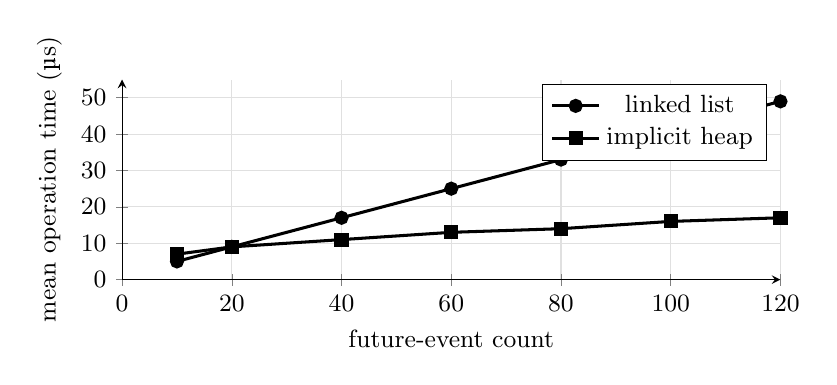
\begin{tikzpicture}
\begin{axis}[
  width=0.82\textwidth,height=0.34\textwidth,
  xmin=0,xmax=120,ymin=0,ymax=55,
  axis lines=left,
  xlabel={future-event count},
  ylabel={mean operation time (\textmu s)},
  xtick={0,20,40,60,80,100,120},
  ytick={0,10,20,30,40,50},
  ticklabel style={font=\small},
  label style={font=\small},
  legend style={font=\small,at={(0.98,0.98)},anchor=north east},
  grid=major,
  major grid style={draw=black!12}
]
\addplot[line width=1.1pt,mark=*] coordinates {
  (10,5) (20,9) (40,17) (60,25) (80,33) (100,41) (120,49)
};
\addlegendentry{linked list}
\addplot[line width=1.1pt,mark=square*] coordinates {
  (10,7) (20,9) (40,11) (60,13) (80,14) (100,16) (120,17)
};
\addlegendentry{implicit heap}
\end{axis}
\end{tikzpicture}
\caption{Mean Insert/Remove Times for Linked Lists and Implicit Heaps}
\label{fig:ext-smpl-event-performance}
\end{figure}

However, replacing the list is not always a net win:
\begin{itemize}
\item same-time FIFO ordering may need secondary keys,
\item event cancellation by event/token is naturally easy on lists,
\item if future-event count is small, list overhead is often acceptable.
\end{itemize}

The chapter recommends measuring typical list size and considering model
reformulation before changing core data structures.

\section{Storages}
\label{sec:ext-smpl-storages}

Storages model finite pools (memory, buffers, etc.) and are conceptually similar
to facilities but capacity-based.

Suggested API:
\begin{itemize}
\item \texttt{s = storage(name, n)},
\item \texttt{r = alloc(s, tkn, m)} (allocate $m$ units; queue if unavailable),
\item \texttt{dealloc(s, k)} (free $k$ units),
\item \texttt{m = avail(s)} (current free units).
\end{itemize}

\begin{figure}[ht]
\centering
\begin{tikzpicture}[>=Latex]
  \draw[line width=1pt] (0,0) rectangle (6.0,3.7);
  \draw[line width=0.8pt] (0,3.0) -- (6.0,3.0);
  \draw[line width=0.8pt] (0,2.3) -- (6.0,2.3);
  \draw[line width=0.8pt] (0,1.6) -- (6.0,1.6);
  \draw[line width=0.8pt] (3.2,0) -- (3.2,3.7);
  \node[font=\small] at (1.6,3.35) {name ptr};
  \node[font=\small] at (4.6,3.35) {queue head};
  \node[font=\small] at (1.6,2.65) {capacity};
  \node[font=\small] at (4.6,2.65) {available};
  \node[font=\small] at (1.6,1.95) {area stats};
  \node[font=\small] at (4.6,1.95) {time mark};
  \node[font=\small] at (1.6,1.25) {alloc count};
  \node[font=\small] at (4.6,1.25) {wait count};
  \node[font=\small] at (3.0,0.45) {storage descriptor};

  \draw[line width=1pt] (7.2,0.6) rectangle (12.4,3.1);
  \draw[line width=0.8pt] (7.2,2.4) -- (12.4,2.4);
  \draw[line width=0.8pt] (7.2,1.7) -- (12.4,1.7);
  \draw[line width=0.8pt] (9.8,0.6) -- (9.8,3.1);
  \node[font=\small] at (8.5,2.75) {token};
  \node[font=\small] at (11.1,2.75) {request $m$};
  \node[font=\small] at (8.5,2.05) {priority};
  \node[font=\small] at (11.1,2.05) {next/prev};
  \node[font=\small] at (9.8,1.15) {wait queue entry};
  \draw[->,line width=0.9pt] (6.1,2.8) -- (7.1,2.8);
\end{tikzpicture}
\caption{Storage Descriptor and Queue Structure}
\label{fig:ext-smpl-storage-structure}
\end{figure}

Key implementation points:
\begin{itemize}
\item descriptor can be built as a facility-structure variant,
\item queue-length and storage-utilization accumulators mirror facility logic,
\item deallocation may admit multiple waiting requests (discipline-dependent).
\end{itemize}

The text discusses FIFO, priority, and best-fit queue variants and the need to
extend reset/trace/report code paths accordingly.

\section{Tables}
\label{sec:ext-smpl-tables}

Tables collect empirical distributions of output variables (response time,
queueing delay, etc.).

\begin{figure}[ht]
\centering
\fbox{%
\begin{minipage}{0.9\textwidth}
\small\verbatimfont
TABLE: response\_time \quad range [0, 40], bins=10\\
count=5000 \quad mean=12.83 \quad stddev=4.27\\
------------------------------------------------------------\\
bin \quad from \quad to \quad freq \quad cum\_freq \quad prob\\
 1 \quad 0.0 \quad 4.0 \quad 112 \quad 112 \quad 0.022\\
 2 \quad 4.0 \quad 8.0 \quad 741 \quad 853 \quad 0.148\\
 3 \quad 8.0 \quad 12.0 \quad 1415 \quad 2268 \quad 0.283\\
 4 \quad 12.0 \quad 16.0 \quad 1328 \quad 3596 \quad 0.266\\
 5 \quad 16.0 \quad 20.0 \quad 804 \quad 4400 \quad 0.161\\
 6 \quad 20.0 \quad 24.0 \quad 363 \quad 4763 \quad 0.073\\
 7 \quad 24.0 \quad 28.0 \quad 148 \quad 4911 \quad 0.030\\
 8 \quad 28.0 \quad 32.0 \quad 66 \quad 4977 \quad 0.013\\
 9 \quad 32.0 \quad 36.0 \quad 18 \quad 4995 \quad 0.004\\
10 \quad 36.0 \quad 40.0 \quad 5 \quad 5000 \quad 0.001\\
\end{minipage}}
\caption{\texttt{smpl} Table Report}
\label{fig:ext-smpl-table-report}
\end{figure}

Definition and entry interface:
\begin{itemize}
\item \texttt{t = table(from, to, n, opt, name)},
\item \texttt{enter(v, t)}.
\end{itemize}

Descriptor fields include lower bound, interval width, option flags, number of
cells, entry count, sums for mean/variance, and underflow/overflow counters.

\begin{figure}[ht]
\centering
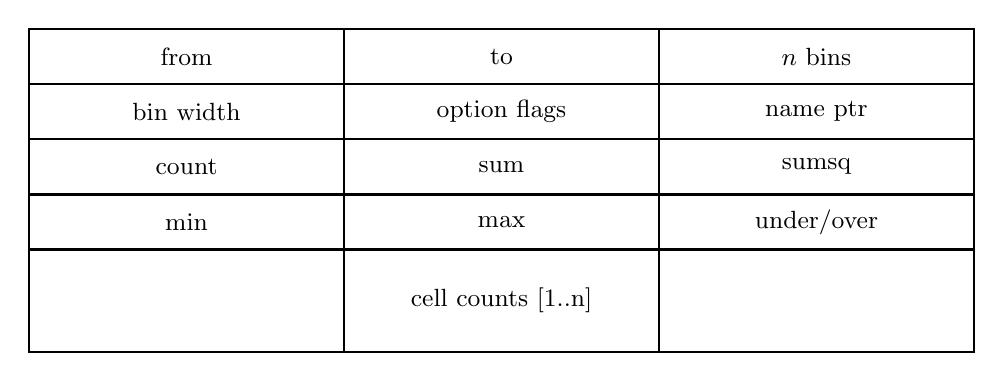
\begin{tikzpicture}
  \draw[line width=1pt] (0,0) rectangle (12,4.1);
  \draw[line width=0.8pt] (0,3.4) -- (12,3.4);
  \draw[line width=0.8pt] (0,2.7) -- (12,2.7);
  \draw[line width=0.8pt] (0,2.0) -- (12,2.0);
  \draw[line width=0.8pt] (0,1.3) -- (12,1.3);
  \draw[line width=0.8pt] (4.0,0) -- (4.0,4.1);
  \draw[line width=0.8pt] (8.0,0) -- (8.0,4.1);
  \node[font=\small] at (2.0,3.75) {from};
  \node[font=\small] at (6.0,3.75) {to};
  \node[font=\small] at (10.0,3.75) {$n$ bins};
  \node[font=\small] at (2.0,3.05) {bin width};
  \node[font=\small] at (6.0,3.05) {option flags};
  \node[font=\small] at (10.0,3.05) {name ptr};
  \node[font=\small] at (2.0,2.35) {count};
  \node[font=\small] at (6.0,2.35) {sum};
  \node[font=\small] at (10.0,2.35) {sumsq};
  \node[font=\small] at (2.0,1.65) {min};
  \node[font=\small] at (6.0,1.65) {max};
  \node[font=\small] at (10.0,1.65) {under/over};
  \node[font=\small] at (6.0,0.65) {cell counts [1..n]};
\end{tikzpicture}
\caption{Table Descriptor}
\label{fig:ext-smpl-table-descriptor}
\end{figure}

On each \texttt{enter()}, the code updates:
\begin{itemize}
\item count, sum, sum-of-squares,
\item min/max,
\item underflow/overflow or selected cell count.
\end{itemize}

The chapter notes that fixed ranges can be inconvenient when location/shape are
unknown; adaptive histogram methods are possible alternatives.

\section{Distributions}
\label{sec:ext-smpl-distributions}

Distribution definition is separated from sampling:
\begin{itemize}
\item \texttt{d = distr(type, p1, p2)},
\item \texttt{v = sample(d)}.
\end{itemize}

This decoupling improves parameterized model setup, debugging, and supports
variance-reduction patterns.

\begin{figure}[ht]
\centering
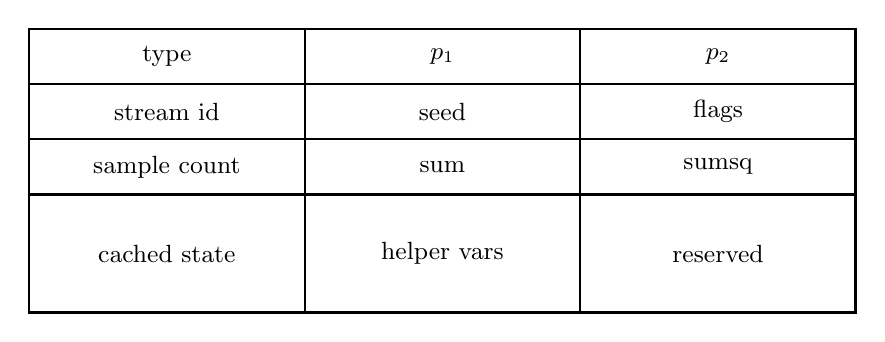
\begin{tikzpicture}
  \draw[line width=1pt] (0,0) rectangle (10.5,3.6);
  \draw[line width=0.8pt] (0,2.9) -- (10.5,2.9);
  \draw[line width=0.8pt] (0,2.2) -- (10.5,2.2);
  \draw[line width=0.8pt] (0,1.5) -- (10.5,1.5);
  \draw[line width=0.8pt] (3.5,0) -- (3.5,3.6);
  \draw[line width=0.8pt] (7.0,0) -- (7.0,3.6);
  \node[font=\small] at (1.75,3.25) {type};
  \node[font=\small] at (5.25,3.25) {$p_1$};
  \node[font=\small] at (8.75,3.25) {$p_2$};
  \node[font=\small] at (1.75,2.55) {stream id};
  \node[font=\small] at (5.25,2.55) {seed};
  \node[font=\small] at (8.75,2.55) {flags};
  \node[font=\small] at (1.75,1.85) {sample count};
  \node[font=\small] at (5.25,1.85) {sum};
  \node[font=\small] at (8.75,1.85) {sumsq};
  \node[font=\small] at (1.75,0.75) {cached state};
  \node[font=\small] at (5.25,0.75) {helper vars};
  \node[font=\small] at (8.75,0.75) {reserved};
\end{tikzpicture}
\caption{Distribution Descriptor}
\label{fig:ext-smpl-distribution-descriptor}
\end{figure}

Each distribution can maintain its own stream seed. That enables:
\begin{itemize}
\item common random numbers across alternatives,
\item antithetic variants (via complemented seed handling).
\end{itemize}

An example type set is proposed:
\texttt{constant}, \texttt{uniform}, \texttt{normal}, \texttt{expntl}
(with Erlang/expntl/hyperexponential selection from mean/stddev relation).

\section{A Run-Time Interface}
\label{sec:ext-smpl-runtime}

The chapter emphasizes that a run-time interface is usually the highest-leverage
extension. In SMPL/PC this role is handled by \texttt{mtr}.

\begin{figure}[ht]
\centering
\begin{tikzpicture}[>=Latex,node distance=1.0cm and 1.5cm]
  \node[draw,rounded corners,minimum width=3.6cm,minimum height=0.9cm] (start) {\texttt{smpl()} startup};
  \node[draw,minimum width=3.8cm,minimum height=0.9cm,below=of start] (i1) {\texttt{init\_mtr()} phase 1};
  \node[draw,minimum width=4.4cm,minimum height=0.9cm,below=of i1] (model) {model defines facilities/parameters};
  \node[draw,minimum width=3.8cm,minimum height=0.9cm,below=of model] (i2) {\texttt{init\_mtr()} phase 2};
  \node[draw,minimum width=3.4cm,minimum height=0.9cm,below=of i2] (loop) {\texttt{cause()} event loop};
  \node[draw,diamond,aspect=1.7,below=of loop] (check) {pause/break/error?};
  \node[draw,minimum width=3.2cm,minimum height=0.9cm,left=2.8cm of check] (mtr) {\texttt{mtr()} command handler};
  \node[draw,minimum width=3.2cm,minimum height=0.9cm,below=of check] (run) {continue execution};

  \draw[->,line width=0.9pt] (start) -- (i1);
  \draw[->,line width=0.9pt] (i1) -- (model);
  \draw[->,line width=0.9pt] (model) -- (i2);
  \draw[->,line width=0.9pt] (i2) -- (loop);
  \draw[->,line width=0.9pt] (loop) -- (check);
  \draw[->,line width=0.9pt] (check) -- node[above,font=\small] {yes} (mtr);
  \draw[->,line width=0.9pt] (mtr) |- (loop);
  \draw[->,line width=0.9pt] (check) -- node[right,font=\small] {no} (run);
  \draw[->,line width=0.9pt] (run) |- (loop);
\end{tikzpicture}
\caption{\texttt{mtr} Initialization and Control Functions}
\label{fig:ext-smpl-mtr-flow}
\end{figure}

Integration points:
\begin{itemize}
\item \texttt{init\_mtr()} called twice from \texttt{smpl} init path
  (before and after facility definition),
\item \texttt{mtr()} called during execution (typically from \texttt{cause()}),
\item optional pause/error hooks.
\end{itemize}

Suggested first features:
\begin{itemize}
\item trace control,
\item report display/reset,
\item parameter display and editing.
\end{itemize}

Parameter support (\texttt{parms} module) uses calls like:
\begin{itemize}
\item \texttt{pdef(num, ptr, name)},
\item lookup helpers by number/pointer.
\end{itemize}

These parameters are then reused by breakpoints, table setup, analysis displays,
and run-time experimentation.

\section{In Conclusion}
\label{sec:ext-smpl-conclusion}

The chapter closes with two practical recommendations:
\begin{enumerate}
\item build a usable run-time interface early, then grow extensions around it;
\item use \texttt{smpl} for small-to-medium models and as a compact simulation
  kernel for specialized tooling.
\end{enumerate}

For large, highly detailed models, process-oriented languages are generally more
natural. Regardless of language, begin with small/high-leverage models early in
design and scale detail incrementally.
